\chapter{Objects and Classes}

\index{object-oriented programming}Object-oriented programming means
different things to different people. In Unicon, object-oriented
programming starts with encapsulation, inheritance, and polymorphism.
These ideas are found in most object-oriented languages as well as many
that are not object-oriented. This and following chapters
present these ideas and illustrate their use in design diagrams and
actual code. Diagrams and code are
alternative notations by which programmers share their knowledge. This
chapter explores the essence of object-orientation and gives you the
concepts needed before you delve into diagrams and code examples. In
this chapter you will learn:
\begin{itemize}\itemsep0pt
\item How different programming languages support objects in different ways
\item To simplify programs by encapsulating data and code
\item The relationship between objects and program design
\item Draw diagrams that show class names, attributes, and methods
\item Write corresponding code for classes and their methods
\item To create instances of classes and invoke methods on those objects
\end{itemize}

\section{Objects in Programming Languages}

Object-oriented programming can be done in any language, but some
languages make it easier than others. Support for objects should not
entail strange syntax or programs that look funny in a
heterogeneous desktop-computing environment. \index{Smalltalk}Smalltalk
has these problems. C++ avoids these programs, but its low-level
machine-orientation is less than ideal as an algorithmic
notation usable by non-experts. \index{Java}Java offers a simple object
model and familiar syntax. The advantages
Unicon has over Java are fundamentally higher-level built-in types,
operations, and control structures.

Many object-oriented languages require that \textit{everything} be done
in terms of objects, even when objects are not appropriate. Unicon
provides objects as just another tool to aid in the writing of
programs, especially large ones. Icon already provides a powerful
notation for expressing a general class of algorithms. The purpose of
object-orientation is to enhance that notation, not to get in the way
of it.

Icon does not support user-defined objects, although its built-in types
have nice object-like encapsulation and polymorphism properties.
Unicon's object-oriented facilities descend from a
package for Icon called \index{Idol}Idol. In Idol, a preprocessor
implemented objects with no support from the underlying Icon runtime
system. In contrast, Unicon has support for objects built-in to the
language. This simplifies the notation and improves the performance of
object-related computations.

Object-orientation adds several general concepts into procedure-based
programming. The single overriding reason for \index{object-oriented
programming}object-oriented programming is to reduce complexity in
large programs. Simple programs can be written easily in any language.
Somewhere between the 1,000-line mark and the 10,000-line mark most
programmers can no longer keep track of their entire program at once.
By using a very high-level programming language, fewer lines of code
are required; a programmer can write perhaps ten times as large a
program and still be able to keep track of things.

As programmers write larger and larger programs, the benefit provided by
\index{very high-level language}very high-level languages does not keep
up with program complexity. This obstacle has been labeled the
``software crisis'', and object-oriented
programming is one way to address this crisis. In short, the goals of
object-oriented programming are to reduce the complexity of coding
required to write very large programs and to allow code to be
understood independently of the context of the surrounding program. The
techniques employed to achieve these goals are discussed below. 

A second reason to consider object-oriented programming is that the
paradigm fits certain problem domains especially well, such as
simulation, and graphical user interfaces. The first well-known
object-oriented language, \index{Simula67}Simula67, certainly had the
domain of simulation in mind. The second pioneering object-oriented
language, Smalltalk, popularized fundamental aspects of bitmapped
graphical user interfaces that are nearly universal today. Three
decades of experience with object-oriented techniques has led many
practitioners to conclude that the concepts presented below are very
general and widely applicable, but not all problems fit the
object-oriented mold. Unicon advocates the use of objects, but this is
a suggestion, not a rule. 

\subsection*{Encapsulation}

The primary concept advocated by object-oriented programming is the
principle of \index{encapsulation}encapsulation. Encapsulation is the
isolation, in the source code that a programmer writes, of a data
representation and the code that manipulates the data representation.
In some sense, encapsulation is an assertion that no other routines in
the program have {\em side-effects\/} with
respect to the data structure in question. It is easier to reason about
encapsulated data because all of the source code that could affect that
data is immediately present with its definition. 

Encapsulation does for data structures what the procedure does for
algorithms: it draws a line of demarcation in the program source code.
Code outside this boundary is irrelevant to
the code that is inside, and vice versa. Communication across the
boundary occurs through a public interface. An encapsulated
data structure is called an object. Just as a set of named variables called
parameters is the interface between a procedure and the
code that uses it, a set of named procedures called methods comprises
the interface between an object and the code that uses it. 

This textual definition of encapsulation as a property of program source
code accounts for the fact that good programmers can write encapsulated
data structures in any language. The problem is not capability, but
verification. To verify encapsulation some languages require
programmers to specify the visibility of every piece of information in
each data structure as {\em public\/} or
{\em private\/}. There are even multiple forms of
privacy (semi-private?). Unicon instead stresses simplicity. 

\subsection*{Inheritance}

In large programs, the same or nearly the same data structures are used
over and over again for myriad different purposes. Similarly,
variations on the same algorithms are employed by structure after
structure. To minimize redundancy, techniques are needed to support
code sharing for both data structures and algorithms. Code is shared by
related data structures through a programming concept called
\index{inheritance}inheritance. 

The basic premise of inheritance is simple: when writing code for a data
structure similar to a structure that is already written,
specify the new structure by giving the differences between it and
the old structure, instead of copying and modifying the old
structure's code. There are times when the
inheritance mechanism is not useful, such as if the two data structures
are more different than they are similar, or if they are simple enough
that inheritance would only confuse things, for example. 

Inheritance addresses multiple programming problems found at
different conceptual levels. The most obvious software engineering
problem it solves might be termed enhancement. During the development
of a program, its data structures may require extension via new state
variables or new operations or both; inheritance is especially useful
when both the original structure and the extension are used by the
application. Inheritance also supports simplification, or the reduction
of a data structure's state variables or operations.
Simplification is analogous to \index{argument culling}\textit{argument
culling}\textit{,} an idea from lambda calculus (don't
worry if this sounds like Greek to you), in that it describes a logical
relation between structures. In general, inheritance may be used in
source code to describe any sort of relational hyponymy, or special
casing. In Unicon the collection of all inheritance relations defines a
directed (not necessarily acyclic) graph. 

\subsection*{Polymorphism}

\index{polymorphism}From the perspective of the writer of related data
structures, inheritance provides a convenient method for code sharing,
but what about the code that uses objects? Since objects are
encapsulated, that code is not dependent upon the internals of the
object at all, and it makes no difference to the client code whether
the object in question belongs to the original class or the inheriting
class. 

We can make a stronger statement. Due to encapsulation,
different executions of code that uses objects to implement an
algorithm may operate on objects that are not
related by inheritance at all. Such code can utilize any objects that
implement the operations that the code invokes. This facility is called
polymorphism, and such algorithms are called generic. This feature is
found in many non-object-oriented languages; in object-oriented
languages it is a natural extension of encapsulation. 

\section{Objects in Program Design}

\index{program design}Another fundamental way to think about objects is
from the point of view of software design. During program design,
objects are used to model the problem domain. The different kinds of
objects and relationships between objects capture fundamental
information that organizes the rest of the program's
design and implementation. Program design includes several other
fundamental tasks such as the design of the user interface, or
interactions with external systems across a network. Additional kinds
of modeling are used for these tasks, but they all revolve around the
object model.

For small, simple, or well-understood software projects, a prose description
may be all the documentation that is needed. The Unified Modeling Language
(\index{UML}UML) is a notation for building software models of larger software
systems for which a prose description alone would be inadequate. It was
invented by Grady Booch, Ivar Jacobson, and James Rumbaugh. In UML, software
models document the purpose and function of a software system.
The advantage of a model is that it conveys
information that is both more precise and more readily understood than
a prose description. UML is used during multiple phases of the software
lifecycle. UML defines several kinds of diagrams, of which we will only
consider four in this book.

\begin{itemize}
\item \textbf{Use case diagrams} show the organization of the
application around the specific tasks accomplished by different users.
\item \textbf{Class diagrams} show much of the static structure of the
application data.
\item \textbf{Statechart diagrams} model dynamic behavior of systems
that respond to external events, including user input.
\item \textbf{Collaboration diagrams} model interactions between
multiple objects
\end{itemize}
These diagrams describe key aspects of many categories of software
applications. The reader should consult the UML Notation Guide and
Semantics documents for a complete description of UML. A good
introduction is given in \textit{UML Toolkit}, by Hans-Erik Eriksson
and Magnus Penker (1998).

A typical application of UML to a software development project uses
these diagrams in sequence. You start by constructing
use case diagrams and detailed descriptions of the different kinds of
users and tasks performed using the system. Then develop class diagrams
that capture the relationships between different kinds of objects
in the system. Finally, construct statechart and
collaboration diagrams as needed to describe the sequences of events
that can occur and the corresponding operations performed by various
objects in response to those events.

Use case and statechart diagrams are important, but their purpose is
to elaborate on an object model described in class diagrams. For this
reason, class diagrams are
presented first, along with the corresponding programming
concepts. Use case diagrams, statecharts, and collaboration diagrams
are discussed in Chapter 12.

\section{Classes and Class Diagrams}

Classes are user-defined data types that model the information and
behavior of elements in the application domain. In Unicon they are
records with associated procedures, called methods. Instances of these
special record types are called objects.  But the language constructs
originated from a need to model application domain concepts, so it is
appropriate to introduce them from that perspective.

Modeling a software system begins with identifying things
that are in the system and specifying how they are related. A class
diagram shows a static view of relationships between the kinds of
elements that occur in the problem domain. A class diagram is a
data-centric, object-centric model. In contrast, a
user-centric view is provided by use cases. \index{class!diagrams}Class
diagrams have several basic components.

Classes are represented by rectangles. A
{\em class\/} denotes a concept of the
application domain that has state information (depicted by named
\index{attribute!class}\textit{attributes}) and/or behavior (depicted
by named \index{operations}operations, or \textit{methods}) significant
enough to be reflected in the model. Inside the rectangle, lines
separate the class name and areas for attributes and operations. Figure
10-1 shows an example class.

\bigskip

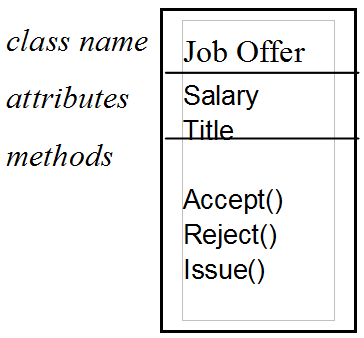
\includegraphics[width=2.3in,height=1.8in]{ub-img/umlclass.png} 

{\sffamily\bfseries Figure 10-1:}
{\sffamily Class Job Offer has two Attributes and Three Methods}

\bigskip

Classes in an object model are
implemented using programming language classes, which are described in
the next section. The degree of separation between the notion of a
class in the model and in the implementation depends on the programming
language. In the case of Unicon, the separation is minimal, because
built-in types such as lists and tables take care of almost all data
structures other than those introduced specifically to model
application domain elements. In the case of C++ or \index{Java}Java,
many additional implementation artifacts typically have to be
represented by classes.

The same class can appear in many class diagrams to capture all of its
relationships with other classes. Different diagrams may show different
levels of detail, or different aspects (projections) of the class
relevant to the portion of the model that they depict. In the course of
modeling it is normal to start with few details and add them gradually
through several iterations of the development process. Several kinds of
details may be added within a class. Such details include:

\begin{itemize}
\item The \index{visibility!within class}\textit{visibility} of
attributes and operations. A plus sign (+) before the attribute name
indicates that the attribute is \index{public}public and may be
\index{reference}referenced in code external to the class. A minus sign
(-) before the attribute name indicates that the attribute is
\index{private}private and may not be referenced in code outside the
class.
\item Types, initial values, and properties of attributes
\item Static properties of the class that will not be relevant at
run-time
\end{itemize}
Attribute names may be suffixed with a colon and a type, an equal sign
and a value, and a set of properties in curly braces. Figure 10-2 shows
two very different levels of detail for the same class. Each level of
detail is appropriate in different contexts.

\bigskip

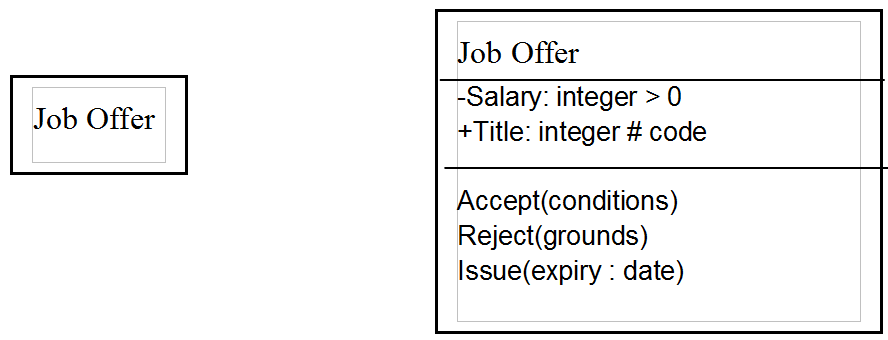
\includegraphics[width=4in,height=1.8in]{ub-img/lodetail.png} 

{\sffamily\bfseries Figure 10-2:}
{\sffamily A Class is Drawn with Different Levels of Detail in
 Different Diagrams}

\bigskip

You can draw rectangles with names of classes inside them all day, but
unless they say something about program organization, such diagrams
serve little purpose. The main point of drawing a class diagram is not
the classes; it is the relationships between classes that are required
by the model. These relationships are called
\index{association}\textit{associations}. In a class diagram,
associations are lines that connect classes. Accompanying annotations
in the diagram convey relevant model information about the
relationships. The details of associations and their implementation are
described in Chapter 10.

\section{Declaring Classes}

\index{class!declaration}In Unicon program code, the syntax of a class
is: 

\iconcode{
class foo(attribute1, attribute2, attribute3, ...) \\
\>   \# procedures (methods) to access class foo objects \\
\ \\
\# code to initialize class foo objects \\
end
}

\noindent
The procedures that manipulate class objects are called
\index{method}\textit{methods}. Methods define a
class' interface from the rest of the program. The
syntax of a method like a procedure: 

\iconcode{
method bar(param1, param2, param3, ...) \\
\>   \# Unicon code that may access fields of a class foo object \\
end
}

Execution of a class method is always associated with a given object of
that class. The method has access to an implicit
\index{variable!implicit}\index{variable}variable called
\index{self}\texttt{self} that is a record containing fields whose
names are the attributes given in the class declaration. Fields from
the \texttt{self} variable are directly accessible by name. In addition
to methods, classes may also contain regular procedure, global, and
record declarations; such declarations have the standard semantics and
exist in the global name space. 

\section{Object Instances}

Like records, \index{instances!class object}instances of a class type
are created with a \index{constructor!class}constructor function whose
name is that of the class. Instances of a class are called objects, and
behave similar to records. The fields of an instance generally
correspond directly to the class attributes. Fields may be initialized
explicitly in the constructor in exactly the same way as for records.
For example, after defining a \texttt{class foo(x, y)} one may write: 

\iconcode{
procedure main() \\
\>   f := foo(1, 2) \\
end
}

In this case \texttt{x} would have the value \texttt{1}, and \texttt{y}
would have the value \texttt{2}, the same as for a record
type. The fields of an object do not have to be initialized by a
parameter passed to the class constructor. Many constructors initialize
objects' fields to some standard value. In this case,
the class declaration includes an \index{initially}\texttt{initially}
section after its methods are defined and before its end. An
\texttt{initially} section is just a special method that is invoked
automatically by the system when it creates each instance of the class.

An \texttt{initially} section begins with the word
\texttt{initially} and an optional parameter list, followed by lines of
code that are executed when an object of that class is constructed.
These lines can assign values to the attributes of the object
being created.

For example, suppose you want an enhanced table type that permits
sequential access to elements in the order they are inserted into the
table. You can implement this using a combination of a list and a
table, both of which would be initialized to the appropriate empty
structure: 

\iconcode{
class taque(L, T) \# pronounced "taco" \\
\>   \# methods to manipulate taques, \\
\>   \# e.g. insert, index, foreach... \\
initially \\
\>   L := [ ] \\
\>   T := table() \\
end
}

\noindent
In such a case you can create objects without including arguments to the
constructor: 

\iconcode{
procedure main() \\
\ \ \ mytaque := taque() \\
end
}

In the absence of an \texttt{initially} section, missing arguments to a
constructor default to the null value. Together with an
\texttt{initially} section, the class declaration looks like a
procedure that constructs objects of that class. You can
write classes with some fields that are initialized explicitly by the
constructor while other fields are initialized automatically in the
\texttt{initially} section. In this case you should either declare the
automatically initialized fields after those initialized in
the constructor, or insert \texttt{\&null} in the positions of the
automatically initialized fields in the constructor. The parameters to
the constructor are exactly in the order they appear in the class
declaration.

This default semantics for constructor parameters is awkward in some
cases, so there is an alternative. The \texttt{initially} section is
really just a special method, and it is allowed to take a parameter
list just like any other method. When an initially section includes a
parameter list, no implicit initialization of objects'
fields is performed. This frees the constructor from having the same
number and order of parameters as the declared class fields. In the
following class, the third field is initialized from constructor
parameter \texttt{x}, overriding the default behavior of initializing
fields in the declared order. This capability becomes important in
large classes with many fields.

\iconcode{
class C(a, b, c) \\
initially(x) \\
\>   c := x \\
end
}

\section{Object Invocation}

Once you have created an object with a class constructor, you manipulate
the object by invoking its class methods. Since objects are
both procedures and data, object \index{invocation!object
method}invocation is a combination of a procedure call and a record
access. The syntax is

\iconcode{
\>   object . methodname ( arguments )}

If an object's class is known, object methods can also
be called using a normal procedure call. This allows object oriented
Unicon code to be called from Icon. Called as a procedure, the name of
a method is prefixed with the class name and an underscore character.
The object itself is always the first parameter passed to a method. In
the absence of inheritance (discussed in the next chapter) if
\texttt{x} is an object of class \texttt{C},
\texttt{x.method(arguments)} is equivalent to \texttt{C\_method(x,
arguments)}.

Although object methods can be called using procedure calls, the field
operator has the advantage that it handles inheritance and polymorphism
correctly, allowing algorithms to be coded generically using
polymorphic operations. Generic algorithms use any objects whose class
provides the set of methods used in the algorithm. Generic code is less
likely to require change when you later enhance the program, for
example adding new \index{subclass}subclasses that inherit from
existing ones. In addition, if class names are long, the field syntax
is considerably shorter than writing out the class name for the
invocation. Using the taque example: 

\iconcode{
procedure main()\\
\>   mytaque := taque() \\
\>   mytaque.insert("greetings",
"hello") \\
\>   mytaque.insert(123) \\
\>   every write(mytaque.foreach()) \\
\>   if mytaque.index("hello") then 
        write(", world") \\
end
}

For object-oriented purists, using the field operator to invoke an
object's methods in this manner is the only way to
access an object. In Unicon, visibility issues such as
``public'' and ``private'' are addressed in an
application's design and documentation. A good
starting point is to consider all fields
``private'' and all methods ``public''. Nevertheless, an object is just a
kind of record, complete with record-style field access.

Direct external access to an object's data fields using
the usual field operator is not good practice, since it violates the
principle of encapsulation. Within a class method, on the other hand,
access to an object's attributes is expected. The
implicit object named \texttt{self} is used under the covers, but
attributes and methods are referenced by name, like other variables.
The taque insert method is thus: 

\iconcode{
method insert(x, key) \\
\>   /key := x \\
\>   put(L, x) \\
\>   T[key] := x \\
end
}

The \texttt{self} object allows field access just like a record, as well
as method invocation like any other object. Using the \texttt{self}
variable explicitly is rare.

\section{Comparing Records and Classes}

The concepts of classes and objects are found in many programming
languages. The following example illustrates Unicon's object model
and provides an initial impression of these
concepts' value. To motivate Unicon's OOP
constructs, our example contrasts conventional Icon
code with object-oriented code that implements the same behavior.

\subsection*{Before objects}

Suppose you are writing some text-processing application such as a text
\index{editor}editor. Such applications need to be able to process
structures holding the contents of various text files. You might begin
with a simple structure like the following: 

\iconcode{
record buffer(filename, text, index)}

\noindent
where \texttt{filename} is a string, \texttt{text} is a list of strings
corresponding to lines in the file, and \texttt{index} marks
the current line at which the buffer is being processed. Icon record
declarations are global; in principle, if the above declaration needs
to be changed, the entire program must be rechecked. A devotee of
structured programming would write procedures to read the buffer
in from a file; write it out to a file; examine, insert and delete
individual lines; and so on. These procedures, along with the record
declaration given above, can be placed in their own source file
(\texttt{buffer.icn}) and understood independently of the program(s) in
which they are used. Here is one such procedure: 

\iconcode{
\# read a buffer in from a file \\
procedure read\_buffer(b) \\
\>   f := open(b.filename) {\textbar} fail \\
\>   b.text := [ ] \\
\>   b.index := 1 \\
\>   every put(b.text, !f) \\
\>   close(f) \\
\>   return \\
end
}

There is nothing wrong with this example; in fact its similarity to the
object-oriented example that follows demonstrates that a good, modular
design is the primary effect encouraged by \index{object-oriented
programming}object-oriented programming. Using a separate source file
to contain a record type and those procedures that operate on the type
allows an Icon programmer to maintain a voluntary encapsulation of that
type. 

\subsection*{After objects}

Here is part of the same buffer abstraction coded in Unicon. The
purpose here is to facilitate a direct comparison with the preceding
record-based example. The example lays the groundwork for a
further object-oriented illustration in the following
chapter. Classes are record types with associated code.
Methods are procedures that are always called in
reference to a particular object (a class instance).

\iconcode{
class buffer(filename, text, index) \\
\>   \# read a buffer in from a file \\
\>   method read() \\
\>   \ \ \ f := open(filename) {\textbar} fail \\
\>   \ \ \ text := [ ] \\
\>   \ \ \ index := 1 \\
\>   \ \ \ every put(text, !f) \\
\>   \ \ \ close(f) \\
\>   \ \ \ return \\
\>   end \\
\>   \# ...additional buffer operations, including method erase() \\
initially \\
\>   if {\textbackslash}filename then read() \\
end
}

This example does not illustrate the full object-oriented style, but
it is a start. The object-oriented version offers encapsulation and
polymorphism. A separate name space for each class's methods allows
shorter names. The same method name, such as \texttt{read()}, can be
used in each class that implements a given operation. This notation is
more concise than is possible with procedures, and it enables an
algorithm to work on objects of any class that implements the
operations required by that algorithm.

Consider the initialization of a new buffer. Constructors allow the
initialization of fields to values other than \texttt{\&null}. In the
example, the \texttt{read()} method is invoked if a filename is
supplied when the object is created. This can be simulated using
records by calling a procedure after the record is created; the value
of the \index{constructor!record}constructor is that it is automatic.
The programmer is freed from the responsibility of remembering to call
this code everywhere objects are created in the client program(s). This
tighter coupling of \index{memory allocation}memory allocation and its
corresponding initialization removes one more source of program errors,
especially on multi-programmer projects. 

The preceding two paragraphs share a common theme:
the net effect is that each piece of data is made responsible for its
own behavior in the system. Although this example dealt with simple
line-oriented text files, the same methodology applies to more abstract
entities such as the components of a
\index{compiler}compiler's grammar.

The example illustrates an important scoping issue. Within class
buffer, method \texttt{read()} makes the regular built-in
function \texttt{read()} inaccessible! Beware of such
conflicts. It would be easy to capitalize the method name to
eliminate the problem. If renaming the method is not an option, as a
last resort you could get a reference to the built-in function
\texttt{read()}, even within method \texttt{read()}, by calling
\texttt{proc("read", 0)}. The function
\texttt{proc()} converts a string to a procedure; supplying a second
parameter of 0 tells it to skip scoping rules and look for a built-in
function by that name.

\section{Summary}

Classes are global declarations that define a record data type and a
set of procedures (methods) that operate on that type. Class instances,
called objects, are normally manipulated solely by calling
the class' methods; such object privacy is a matter of
design, documentation, and
convention. All methods execute within an
object of interest, whose fields and methods are visible
without the record dot notation, in a
class scope that is introduced in between the local and global scopes.




\bigskip
